% 第 3 章 设计与实现方案
% 本章引用键：fips203, kyber2018, kyberslash, clangover, dudect, rtlf, ctgrind, microwalk, binsec
% 合并进 main.tex 时，导言区需提供：algorithm, algpseudocode, listings
\floatname{algorithm}{算法}
\renewcommand{\algorithmicrequire}{\textbf{输入：}}
\renewcommand{\algorithmicensure}{\textbf{输出：}}
\renewcommand{\lstlistingname}{代码}
\lstset{
  language=C,
  basicstyle=\ttfamily\footnotesize,
  numbers=left,
  numberstyle=\tiny,
  columns=fullflexible,
  keepspaces=true,
  frame=single,
  xleftmargin=2.2em,
  framexleftmargin=1.6em,
  aboveskip=6pt,
  belowskip=6pt,
  showstringspaces=false
}

\section{设计与实现方案}

这一章讲检测平台怎么搭。起点是解封装流程本身：先弄清哪些步骤接触秘密，测量、判定、定位和防护才有依据。要分辨的差异只有几十纳秒，单次测量看不出来，所以测量、统计和定位必须一起设计。下面从解封装流程与泄漏面讲起，按测量、判定、定位、防护的顺序说明每一步的做法与取舍。

\subsection{解封装流程与泄漏面}
% A-17--A-23 机制与定位证据，A-22 90 格
% B-06 90 格分解

ML-KEM 解封装在 Fujisaki--Okamoto 变换下完成解密、重加密、比较与隐式拒绝四步计算，每一步接触的秘密并不相同。解密接触私钥与解出的消息，重加密把消息重新送进编码、数论变换、压缩与序列化，比较同时接触真密钥与假密钥，隐式拒绝决定失败时输出什么。把这条链笼统称为“实现有侧信道”，后续的测量与定位就没有明确的检查对象。泄漏面必须按步骤拆开，才可能落到函数与指令。\cite{fips203}

\begin{algorithm}[H]
\caption{ML-KEM 解封装与隐式拒绝}
\label{alg:decaps}
\begin{algorithmic}[1]
\Require 密文 $c$（1088 B），解封装密钥 $dk=(dk_{\mathrm{PKE}},h,z)$
\Ensure 共享密钥 $K$（32 B）
\State $m' \gets \mathrm{K\text{-}PKE.Decrypt}(dk_{\mathrm{PKE}}, c)$ \Comment{解密，使用私钥}
\State $(K', r') \gets G(m' \parallel h)$ \Comment{派生候选密钥与重加密随机数}
\State $c' \gets \mathrm{K\text{-}PKE.Encrypt}(dk_{\mathrm{PKE}}, m', r')$ \Comment{重加密}
\State $\bar K \gets J(z \parallel c)$ \Comment{隐式拒绝的假密钥}
\State $K \gets \mathrm{Select}(c' = c,\ K',\ \bar K)$ \Comment{常数时间比较与掩码选择}
\State \Return $K$
\end{algorithmic}
\end{algorithm}

算法 1 梳理了标准规范中接触敏感秘密数据的五个核心逻辑阶段。但在实际工程落地中，标准伪代码并不规定具体的实现细节（例如消息编码采用逐系数写入还是向量化批量处理，多项式压缩采用原地变换还是缓冲区拷贝），不同的实现架构决定了潜在的敏感分支会落在哪个函数与指令中。因此，后续排查不仅以这五个算法步骤作为逻辑划分，更必须深入到具体的 C 语言函数与最终编译出的机器指令层。

第 1 步解密的秘密是私钥与解出的消息。消息解码函数里的一次整数除法，就是 M2 三处秘密除法中的第一处。除法指令的时延随操作数变化时，私钥系数会进入耗时。\cite{kyberslash} 第 3 步重加密把消息重新送进消息编码、数论变换、压缩与序列化：M1 的分支出现在消息编码，编译器把源码中的掩码选择还原成按位测试后条件跳转。M2 的另两处除法出现在多项式压缩与向量压缩。M3 的人工秘密下标也插在这条路径上。\cite{clangover}

第 4 步比较对应 M4 的提前返回夹具。第 5 步的隐式拒绝必须由常数时间比较与掩码选择完成。只要实现让分支或提前返回依赖比较结果，成功与失败两条路径就可以从耗时上分开，隐式拒绝的设计目的就落空。图~\ref{fig:decaps} 把这条对应关系画在同一张流程图上。M5 不挂在单独一步上，它作为整条链的阴性对照。图中“是/否”表示密钥的逻辑选择，实际实现同时计算拒绝密钥，再用掩码选择输出。

\begin{figure}[htbp]
\centering
\includegraphics[width=0.94\textwidth]{assets/fig31.pdf}
\caption{ML-KEM 解封装流程与常数时间选择}
\label{fig:decaps}
\end{figure}

泄漏来源分为六类，每一类都在解封装链上有明确的作用点。

\begin{enumerate}
\item 敏感条件分支：消息位或比较结果决定执行路径，两条路径的指令数或访存不同。
\item 提前返回：比较在发现第一个不同字节时结束，函数返回时刻取决于失配位置。
\item 可变时间比较与可变时延指令：逐字节比较提前退出，或整数除法等指令的时延随操作数变化。
\item 秘密下标访存：查表下标含秘密位，不同下标落在不同缓存行。
\item 数据相关循环：循环次数或迭代上界随秘密变化。
\item 异常处理路径：成功与失败走不同的分支、日志与返回码。
\end{enumerate}

六类来源的检查手段不同：前三类靠反汇编与秘密标记，第四类靠执行轨迹与秘密的互信息，第五类靠控制流核对，第六类靠泄漏渠道审计。工具放在 3.7 节，这里只固定分类口径，同一现象按统一名称登记。

这六类按“秘密以什么方式影响执行”划分检查口径，同一条指令可同时属于两类。例如逐字节比较既是可变时间比较，也可能带提前返回。排查时按“最早把秘密带入可观测差异的那一步”归类，同一现象在两格内只登记一次。归类规则写进排查表的使用说明，换人核对时按同一口径。题面列出的六类来源覆盖了从控制流、访存到错误处理的主要通道。功耗、电磁这类物理通道属评估边界外项目，平台只测时间。

把这六类来源分别放到三个实现、五个解封装步骤上，就得到 $3\times5\times6=90$ 格的全流程排查表。五个步骤是解密、哈希派生、重加密、密文比较与隐式拒绝。三个实现是 M1、M2 与 M5，人工夹具 M3、M4 不进入这张表。每一格只允许四种判定：存在、不存在、不适用、未检查。判定规则在排查前写定：判“存在”必须给出可指认的函数、指令或源码位置以及触发它的输入。判“不存在”必须写明用了哪种检查、覆盖了哪些输入。判“不适用”要求该机制在这一步骤上不可能出现，例如该步骤没有异常处理。判“未检查”单列，不得并入阴性。

逐格结论与证据编号见 4.5 节与附录 D，本节只定义方法与判定规则。

每一格的记录不只写判定，还要写证据。字段包括：实现与产物摘要、步骤、来源类别、判定、函数名或指令地址、触发输入、使用的检查手段、证据编号。判“存在”的格子必须有触发输入。没有触发输入的“存在”只能算“疑似”，在汇总时降级为“未检查”。判“不存在”的格子要写覆盖了哪些输入。只跑过一个输入的阴性不足以支撑“不存在”。这套字段让 90 格既是排查表，也是审计清单：换一个人按同样字段复核，结论应当一致。

五步的划分比算法 1 多出”哈希派生”一步。算法 1 把派生与重加密写在一起，排查时若合并，哈希路径上的问题会被记到重加密名下。拆开后，派生步骤只检查哈希调用本身，重加密步骤只检查编码、变换、压缩与序列化。这使排查表多出一列，但定位结论可以直接落到”哪一步、哪个函数”。

按步骤拆开后，M1 的消息编码分支与 M2 的压缩除法分属不同步骤；若合并归入”重加密有问题”，定位只能停在重加密这一层，修复也无法核对到底改了哪条指令。90 格把每一格绑定到”实现 × 步骤 × 来源”，任何一格判”存在”都附一个可复核的代码位置，修复后同一格可以被复查为”不存在”。修复后按同一张表复查，目标格从”存在”变为”不存在”，其余格保持不变，修复的副作用也能被看见。通过排查前为每个实现准备五步的证据口径、排查后维护 90 条带证据编号的记录，定位结论可以追溯。

\subsection{泄漏机理与攻击可行性}
% A-01--A-08 主结果，A-13 dudect M2
% B-01 效应占比，B-07 样本账

输入类与重复调用遵循第 1.2 节的威胁模型：评估者选择密文类别与调用次数，观察完整解封装耗时。主检验比较两类合法等长密文的耗时分布，并报告样本量与检测预算。

一次解封装的耗时可以写成
\begin{equation}\tag{3.1}
T = T_0 + \delta(\text{secret}) + \text{noise},
\end{equation}
其中 $T_0$ 是公开路径的平均耗时，$\delta$ 是秘密相关部分，noise 来自调度、频率、缓存与地址对齐。M1 未修版本在 57 µs 的均值上只多出 32.3 ns，$\delta/T_0$ 约为 0.06\%。本地锁频压住的是噪声中的频率项，压不住 $\delta$ 本身。要在噪声里分出 $\delta$，只能靠大样本与预注册检验。每类 10,000 次、三次独立运行，是把可检出下界压到几十纳秒量级的直接原因（3.5、3.6 节）。图~\ref{fig:adversary} 把观测模型画成四段链：攻击者选择输入、解封装预言机返回耗时、样本进入统计判定、结论绑定预算；泄漏方程见式 (3.1)。 % A-01 % B-01 % B-07

主类对在固定解封装密钥对 $(pk,dk)$ 下构造。由公开种子派生封装随机数，分别将内部 32 字节消息 $m'$ 固定为全 0（\texttt{0x00...00}）和全 1（\texttt{0xFF...FF}），再经合法封装流程生成长度均为 1088 字节的有效密文 $C_0$ 与 $C_1$。在 FO 变换中，无论密文是否被篡改，解封装都会先解密出 32 字节候选消息 $m'$ 并执行重加密。固定公钥与随机数种子、仅将内部消息 $m'$ 设为全 0（\texttt{0x00...00}）与全 1（\texttt{0xFF...FF}），能够保证外部密文长度合法且执行路径一致，同时最大化触发内部消息编码、压缩和比较步骤中依赖比特 0/1 的分支或指令耗时差异。选全 0 与全 1，是因为它们让内部消息的每一位在两类输入间系统性取反，覆盖“全不置位”与“全置位”两个极端，且与 FO 重加密中逐位处理的编码路径对应，是最能暴露“消息位是否影响执行路径”的等长合法输入对。两类输入在解封装时均经过解密、重加密、密文比较和隐式拒绝选择代码；固定密钥、种子派生流程与长度一致，实验自变量是预设消息位，密文其他字段由标准算法随之派生。

\begin{algorithm}[H]
\caption{攻击者的计时观测与可区分性实验}
\label{alg:distinguish}
\begin{algorithmic}[1]
\Require 解封装预言机 $\mathcal{O}$，两类合法等长密文 $C_0,C_1$，每类样本 $n$，显著性 $\alpha$
\Ensure 可区分 / 未检出（附效应量与区间）
\For{$b \in \{0,1\}$}
  \For{$i=1$ \textbf{to} $n$}
    \State $c \gets \mathrm{Sample}(C_b)$ \Comment{由公开种子派生，长度合法}
    \State $t_{b,i} \gets \mathrm{Time}(\mathcal{O}(c))$ \Comment{只测一次完整解封装}
  \EndFor
\EndFor
\State $\Delta \gets \mathrm{mean}(t_0) - \mathrm{mean}(t_1)$
\State $CI \gets \Delta$ 的 95\% 置信区间
\If{$CI$ 不含 0}
  \State \Return 可区分 $(\Delta, CI)$
\Else
  \State \Return 未检出 $(\Delta, CI, \mathrm{MDE})$
\EndIf
\end{algorithmic}
\end{algorithm}

算法 2 给出了在既定样本量预算与观测模型下，评估两类输入密文时间分布差异性的判定流程。

\begin{figure}[htbp]
\centering
\includegraphics[width=0.98\textwidth]{assets/fig32.pdf}
\caption{攻击者观测模型}
\label{fig:adversary}
\end{figure}

四类机理可以用最小形态写清楚。代码 1 到代码 4 只保留结构，不写完整实现，也不构成可直接复用的攻击代码。

\noindent\begin{minipage}{\linewidth}
\begin{lstlisting}[caption={秘密相关分支的最小形态},label={code:branch}]
/* 消息位决定走哪条路径；两条路径的指令数或访存不同 */
int16_t select_coeff(const uint8_t *msg, size_t i)
{
    if ((msg[i / 8] >> (i % 8)) & 1)
        return COEFF_ONE;
    return 0;
}
\end{lstlisting}
\end{minipage}

代码 1 对应 M1 的消息编码：源码本用掩码，编译器在特定选项下把它还原成按位测试后条件跳转。边界是：这段代码用于说明机制，上游源码的原样写法按仓库快照核对。分支是否出现取决于编译器与优化选项，必须看实际产物。

\noindent\begin{minipage}{\linewidth}
\begin{lstlisting}[caption={秘密相关除法的最小形态},label={code:divide}]
/* x 来自解密消息；整数除法的时延可能随操作数变化 */
int16_t compress_coeff(int16_t x)
{
    return (int16_t)((((int32_t)x << 4) + (Q / 2)) / Q);
}
\end{lstlisting}
\end{minipage}

代码 2 对应 M2 的三处除法，$Q$ 为公开模数。边界是：除法是否真的有可测时延取决于处理器与编译选项。本作品在特定产物上定位到三处整数除法，但端到端与热点微基准都未检出。

\noindent\begin{minipage}{\linewidth}
\begin{lstlisting}[caption={秘密下标查表的最小形态},label={code:lookup}]
/* 下标来自消息位；不同下标落在不同缓存行 */
int16_t lookup_coeff(unsigned secret_index)
{
    static const int16_t table[16] = { /* 16 个公开常数 */ };
    return table[secret_index & 15];
}
\end{lstlisting}
\end{minipage}

代码 3 对应 M3 的人工校准夹具：查表插在常数时间基线的重加密路径上，开启查表版（on版）与消除查表版（off版）的输出逐字节相同，用于检验工具对秘密下标访存的识别能力。

\noindent\begin{minipage}{\linewidth}
\begin{lstlisting}[caption={提前返回比较的最小形态},label={code:early}]
/* 发现第一个不同字节就返回；耗时取决于从哪里开始不同 */
int compare_bytes(const uint8_t *a, const uint8_t *b, size_t len)
{
    for (size_t i = 0; i < len; i++)
        if (a[i] != b[i])
            return 0;
    return 1;
}
\end{lstlisting}
\end{minipage}

代码 4 对应 M4 的比较夹具：脆弱实现（vulnerable版）发现首个不同字节即返回，常数时间实现（ct版）逐字节异或累积并在固定长度结束后统一判断。两版输出保持逐字节相同。

可区分性是侧信道分析链中的一环；机制存在、计时可区分与攻击可利用分别评估，各对应一个证据层。M2 是典型例子：三处除法在定位层稳定命中，端到端完整解封装与除法热点微基准均未检出；同一份实现中，dudect 的最大 $t$ 还落在已修复版上。证据因此按机制、计时与可利用性分层登记。

主类对只让解密消息的位全 0 或全 1 不同，其他条件相同。这样两类的路径长度接近，差异只能来自消息位。随机密文、逐字节篡改、格式破损与截断属于族外对照：随机密文检验一般路径，篡改与破损检验隐式拒绝，截断检验公开长度检查。族外对照单独登记、不参与 Holm 家族的多重校正：输入路径长度或返回位置不同，混入主家族会把路径差异误读为秘密泄漏；族外对照用于检查主类对之外的输入行为。

\begin{table}[H]
\centering
\caption{攻击可行性对照}
\label{tab:attack}
{\footnotesize
\begin{tabularx}{\textwidth}{|>{\raggedright\arraybackslash}p{2.2cm}|>{\raggedright\arraybackslash}X|>{\raggedright\arraybackslash}X|>{\raggedright\arraybackslash}X|}
\hline
机制 & 攻击者需要的观测 & 本作品做到哪 & 离密钥恢复还差什么 \\
\hline
秘密分支（M1） & 同一密文类下，消息位不同导致耗时不同 & 本地锁频、完整解封装、三次运行可区分（+32.3 ns） & 选择密文构造、逐位消息恢复、纠错与多轮查询。本作品不做 \\
\hline
秘密除法（M2） & 除法操作数不同导致耗时不同 & 定位层稳定命中三处除法。端到端与热点微基准未检出 & 更大样本量、针对除法的输入类、远程噪声下的可观测性。本作品不做 \\
\hline
秘密下标（M3） & 不同下标落在不同缓存行导致耗时不同 & 人工夹具上动态检查与轨迹互信息命中。计时层未检出 & 共驻缓存攻击模型、缓存驱逐与观测。本作品不做 \\
\hline
提前返回（M4） & 比较从第几个字节开始不同导致耗时不同 & 32 B 夹具上脆弱版可区分，常数时间版不可区分 & 完整 KEM 比较路径、远程噪声、逐字节恢复。本作品不做 \\
\hline
阴性对照（M5） & 若存在机制，应能被工具或计时发现 & 三种动态模式 0 报告、有界验证无秘密相关控制流、计时未检出 & 不是“无泄漏”的证明。需要更大预算与其他工具 \\
\hline
\end{tabularx}
}
\end{table}

M2 的三处除法在定位层命中，端到端合并差 $+4.58$ ns、区间 $[-3.08, 12.25]$ 含 0，热点微基准合并差 $+0.044$ ns、区间含 0。表~\ref{tab:attack} 将定位、计时与攻击所需条件并列，说明三类证据各自回答的问题。

\subsection{总体架构与证据分层}
% A-22、A-24 证据分层与工具矩阵
% B-05、B-06 矩阵与排查分解

平台的价值在于把冻结计划、被测对象、测量、分析、登记串成一条可追溯的流水线。任一环节的工具可替换，“结论必须能回到运行编号与证据编号”这条约束固定不变。

\begin{figure}[htbp]
\centering
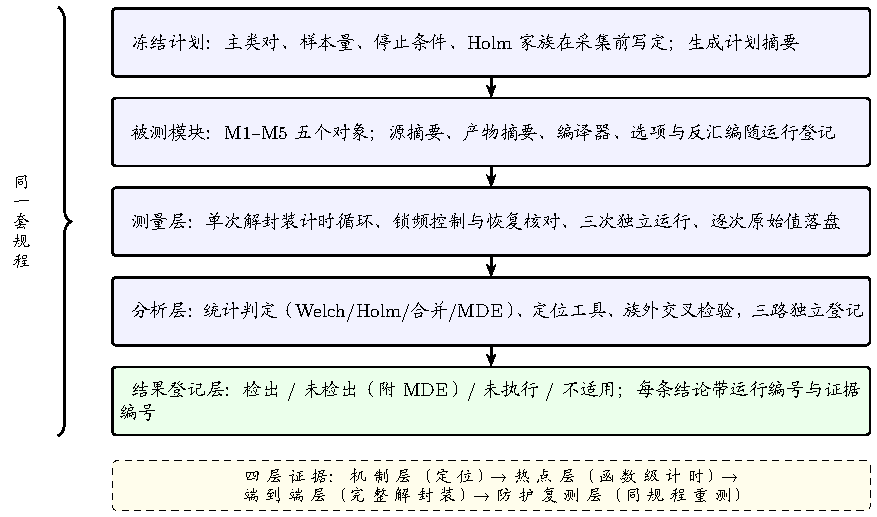
\includegraphics[width=0.96\textwidth]{assets/fig3.pdf}
\caption{平台总体架构与证据分层}
\label{fig:architecture}
\end{figure}

冻结计划层在采集前写定主类对、样本量、停止条件与 Holm 家族，并生成计划摘要。测量层每次运行校验摘要，防止采集开始后改规则。被测模块层固定五个对象，记录源摘要、产物摘要、编译器、选项与反汇编，判定与计时使用同一个二进制。测量层执行计时循环与锁频控制，每次调用逐次落盘，失败样本单列。分析层三路独立：统计判定回答“是否可区分”，定位工具回答“哪里依赖秘密”，族外检验回答“换个统计口径是否还成立”。结果登记层把每条结论写成四种状态之一，附运行编号与证据编号，未执行与不适用不并入阴性。图~\ref{fig:architecture} 给出五层的顺序与共用的规程。

五层的顺序按防篡改逻辑排列：计划在最前，后续每一层都只能按计划执行。被测模块在测量之前固定，避免测到一半换产物。分析在测量之后，三路互不覆盖。登记放在末端，任何一条结论都必须带运行编号与证据编号。探索性分析按族外观察或后续工作登记，进入主家族需预先纳入检验计划。

登记层的每条记录都有唯一编号，编号由运行编号、证据编号与计划版本三段拼接。引用时只写编号，不再复述结论。这样第 4 章引用第 3 章的方法时，读者可以顺着编号回到原始记录，而不必在两章之间寻找同一句话。

计划摘要还有一个副作用：任何一次运行都能被独立复算。审计者拿到计划文件、运行记录与原始值，可以重算摘要、重跑统计、核对恢复记录，独立复算不依赖报告叙述。被拒绝的运行同样登记，编号连续，审计记录包含“尝试过但没通过”与成功的样本。

四层证据是登记时的四个层次。机制层看源码、反汇编与动态标记能否指出秘密相关行为。热点层看函数级微基准或工具定位到的热点是否显示时间差。端到端层看完整解封装的类对检验。防护复测层看修复后在同一规程下重测的结果。

四层的判据不同：统计层的“检出”是预注册检验拒绝，“未检出”是预先规定的检验未拒绝零假设。定位层的“检出”是工具稳定命中且能归因到函数、指令或源码行，动态工具的“未检出”只覆盖执行过的输入。防护复测层的“检出”是修复后目标机制仍在或计时差仍可区分。四种状态互斥：检出、未检出、未执行、不适用。未执行是没做，不适用是机制与步骤的组合不可能出现。

四种状态按判定依据区分：“未检出”附样本、检验与 MDE；“未执行”记录缺少的条件与受影响条目。附录 A 与第 6.2 节列出这些记录，不计入阴性。

将证据划分为机制定位层与端到端计时层，能够清晰解释 M2“定位工具命中、但计时检验未检出”的现象：前者说明二进制代码中确实存在依赖秘密的除法指令，后者说明该指令引入的微弱时延在完整解封装的噪声背景下未被当前样本量分辨出来。两者从不同维度刻画同一实现，并不矛盾。

\subsection{被测对象与模块设计}
% A-17--A-21 对象定位，A-26、A-27 优化与架构
% B-11 优化矩阵

本作品选取的五个被测对象分别承担三类评估角色：真实历史漏洞案例（M1、M2）用于检验平台在真实密码库编译产物上的漏洞检出能力与补丁核验能力；人工构造靶标（M3、M4）用于检验各定位与计时工具对特定侧信道机理的识别灵敏度；常数时间参考实现（M5）作为阴性对照，用于检验平台在合规实现上是否会产生误报（假阳性）。表~\ref{tab:objects} 列出五个对象的固定版本、编译条件、泄漏机制与修复或对照，表中的提交号仅用于定位历史版本。

\begin{table}[H]
\centering
\caption{被测对象与编译条件}
\label{tab:objects}
{\small
\begin{tabularx}{\textwidth}{|>{\raggedright\arraybackslash}p{0.9cm}|>{\raggedright\arraybackslash}X|>{\raggedright\arraybackslash}p{3.4cm}|>{\raggedright\arraybackslash}p{4.2cm}|>{\raggedright\arraybackslash}p{3.3cm}|}
\hline
模块 & 对象与固定版本 & 编译条件 & 泄漏机制 & 修复或对照 \\
\hline
M1 & liboqs 0.10.0，ML-KEM-768 初始公开草案的可移植 C 路径 & clang 18.1.3，面向体积优化（-Os），关闭向量化与 AVX2 分发 & 编译器把消息编码还原为按位测试后条件跳转 & 官方修复提交 982c762 \\
\hline
M2 & pq-crystals Kyber768 参考实现，未修快照 a621b8d & clang 18.1.3，极致体积优化（-Oz） & 三处秘密被除数除以公开模数 & 官方修复提交 272125f。另一提交 dda29cc 只修第一处 \\
\hline
M3 & 基于 mlkem-native，在消息编码路径插入秘密下标查表 & 与 M5 相同 & 秘密下标访存（人工埋入） & 开启查表版（on版）/消除查表版（off版），输出逐字节相同 \\
\hline
M4 & 独立 32 B 比较函数 & 独立编译，i386，-O1 & 发现首个不同字节即返回（人工埋入） & 脆弱实现（vulnerable版）/常数时间实现（ct版） \\
\hline
M5 & mlkem-native 固定版本 b3ba7b3 & 参考 C 路径 & 设计为常数时间 & 阴性对照 \\
\hline
\end{tabularx}
}
\end{table}

M1 与 M2 是真实历史案例。M1 的可移植 C 路径在特定编译器与选项下被还原出分支，M2 的历史 Kyber768 参考实现出现三处秘密除法\cite{kyber2018}。两者都有上游修复可比对，因此能同时回答”检出”与”修复后是否消失”。真实案例的局限在于不能任意控制变量：M1 的构建要额外处理运行时分发，M2 的除法只在特定优化级别出现。

M3 与 M4 是人工校准夹具：M3 在常数时间基线的消息编码路径上插入秘密下标查表，M4 用独立的 32 B 比较函数对比提前返回与常数时间两个版本。两版输出逐字节相同，确保校准的是检测器而不是算法语义。人工夹具回答“工具能不能识别目标机制”；“真实库有没有这个缺陷”由真实案例回答。M5 是阴性对照，设计为常数时间，用来估计工具误报。它在七种工具上的误报为 0，该数字登记这七种工具在本对象与这些输入上的结果；常数时间属性另行核验。

人工夹具的设计要点是”只差目标机制”。M3 的开启查表版（on版）与消除查表版（off版）除查表外完全相同，M4 的两个版本除比较方式外完全相同。输出逐字节相同是先决条件，否则计时差异可能来自语义变化而不是泄漏。人工夹具只能覆盖一种机制，不能代表完整解封装的交互。真实案例补上这一点，但真实案例又不能任意开关机制。三类角色合起来，才覆盖”能检出、能识别、不误报”三个问题。

选择历史 Kyber768 而不是最终标准作为 M2 的对象，是因为 KyberSlash 的两处修复提交落在历史代码上。最终标准改了消息编码与压缩的实现细节，同一机制在最终标准里可能已被间接消除。检验平台能否识别该机制，须在机制存在的版本上进行；M2 的对象描述按历史快照登记为 Kyber768。

判定用的二进制与计时用的二进制必须相同。每次运行记录源摘要、产物摘要、编译器版本、选项与反汇编摘要。采集前核对产物摘要，分析时再核对一次；M1 前期封存批次的来源在运行台账中单独标注。分析脚本拒绝没有摘要的输入，避免手工拷入的数据混入统计。

复现历史案例时，有两项编译配置直接决定待测机制是否真正执行。第一，liboqs 会根据 CPU 能力在运行时选择实现；只调整可移植构建选项，仍可能调用 AVX2 优化路径。因此需要同时关闭 AVX2 指令与对应实现开关，再用反汇编确认调用的是目标 C 函数。第二，M2 在本作品选定的 \texttt{-Oz} 体积优化构建中保留硬件 \texttt{div} 除法指令，换用其他优化配置可能被改写为乘法与移位。采集程序因此记录并核对二进制摘要，产物一变就拒绝沿用旧结论。

版本固定还意味着第三方代码只读：上游文件不改，修复以补丁形式叠加，补丁前后的源摘要与产物摘要都登记。这样一来，“官方修复”与“团队修改”不会混在同一次构建里，审计时可以分别核对。两次构建核对都进运行记录，缺一份就不能出具判定。

M1 的对象按 FIPS 203 初始公开草案登记。草案与正式版的密钥生成采用不同的哈希输入，正式版增加了用于区分参数集的域分隔字节。KeyGen 测试专门核对这一标准演进差异，版本不匹配与算法实现错误分开登记。对象版本必须与期望向量一致，功能结果和侧信道结论才能正确解释。

在侧信道评估中，若用未优化的调试版本做动态定位，却用高优化的发布版本做计时采样，两者的机器码形态往往并不一致，结论也无法相互印证。因此，平台通过计算并校验二进制文件的 SHA-256 摘要，强制要求动态定位、反汇编检查与高精度计时必须针对同一份编译产物执行，确保每一条测试记录都能精确追溯到对应的可执行文件。

\subsection{测量层设计}

测量层的目标，是让每次调用的耗时都可复算、可追溯，且每一步的边界都清楚。受控测量围绕这一目标采用六项措施：将采集进程绑定到 CPU2 或 CPU6；关闭睿频并将频率上下限请求设为 4.30 GHz；将调速策略设为性能模式；在窗口外预热 100 次；按公开种子随机交错两类密文；将内存分配、日志和 I/O 全部移出计时窗口。各项配置及频率探针随运行保存，结束后恢复原设置。

% A-29 锁频对照，A-30 计时精度，A-31 运行批次
% B-07 样本账，B-08 运行批次合计

目标按“测到真实的单次耗时”设定：计时窗口里多放一次内存分配或一行日志，32 ns 量级的效应就会被淹没。窗口外少做一次预热，前几百次调用会把缓存与分支预测的冷启动写进均值。

\begin{algorithm}[H]
\caption{单次解封装的计时循环}
\label{alg:timing}
\begin{algorithmic}[1]
\Require 被测二进制，类别集合 $\mathcal{C}$，每类样本 $n$，种子 $s$，CPU 核 $k$
\Ensure 逐次记录与元数据
\State 生成输入流。按 $s$ 做可复现的类别乱序。记录输入流摘要
\State 在计时窗口外预热 100 次
\For{每个（类别，密文）按乱序}
  \State $t_0 \gets \mathrm{Clock}()$
  \State $\mathrm{Decaps}(\text{密文})$ \Comment{窗口只包住一次完整解封装}
  \State $t_1 \gets \mathrm{Clock}()$
  \State 写入运行编号、实现、类别、序号、$t_1-t_0$ 与单位
\EndFor
\State 记录元数据：源摘要、产物摘要、编译器、选项、时钟、频率、CPU、计划摘要
\State 失败样本单列。不删普通长尾。不扣读钟开销
\end{algorithmic}
\end{algorithm}

算法 3 规定了单次解封装的高精度纳秒级耗时采样与原始数据落盘流程；采集后的时间序列数据送入统计层进行显著性检验，测量环境的稳定性则由算法 4 提供的锁频机制提供保障。

计时循环还有一个容易忽略的约束：每次调用后返回值必须被用掉。编译器可能把没有用到的解封装调用整个删掉，或者把循环折叠成一次调用。把返回值写入一个随后被校验的累加器，才能保证每次调用真的发生，这增加了一次内存写，但它在计时窗口之外。

输入生成、内存分配、结果处理、日志与 I/O 全部在窗口外，窗口内只有一次完整解封装。类别乱序按种子生成，避免”先测完 A 再测 B”时环境漂移造成假差异。预热 100 次让缓存与分支预测进入稳定状态。原始值全量落盘，普通长尾保留，异常样本规则在计划中预先写定，不在看到数据后删点。每次运行产生的逐次记录与样本量同阶，存储与整理成本随运行次数线性增长，但任何一次判定都能从原始值复算。

读钟开销按原始值保留：扣掉一个常数不改变两类均值差，却会让原始值失去可复算性。读钟开销约 17.4 ns，已在分辨率说明里单列。窗口内的调用返回值必须被用掉，窗口外的日志与内存分配全部移走。这两条比“换一个更快的时钟”更能决定数据质量。预热次数在计划里写定：预热负责让缓存与分支预测进入稳定状态，超过稳定点后分布不变，多余预热只增加计算资源开销。

\begin{algorithm}[H]
\caption{锁频控制与恢复核对}
\label{alg:frequency}
\begin{algorithmic}[1]
\Require 目标频率 $f_0=4.30$ GHz，CPU 核 $k$，探针次数 $m=20$
\Ensure 放行 / 拒绝。进入、采中、退出三段记录
\State 保存睿频开关、调速策略、能效偏好与频率上下限的原始快照
\State 关闭睿频。调速策略设为性能模式。能效偏好设为性能模式。频率下限与上限均设为目标频率
\State 用绑核工具把被测进程绑定到核 $k$
\State 等待 1.0 s
\For{$i=1$ \textbf{to} $m$}
  \State 读当前频率。间隔 50 ms
\EndFor
\If{全部 $|f-f_0|/f_0 \le 2\%$ 且 $\max-\min \le 50000\text{ kHz}$}
  \State 放行
\Else
  \State 拒绝，恢复快照，记录原因
\EndIf
\State 采集结束后恢复快照。读取并比较恢复核对结果
\end{algorithmic}
\end{algorithm}

算法 4 建立了采集前后的 CPU 频率工作点锁定与恢复校验规程，确保多次独立实验在统一的硬件频率基准下开展。

探针的判据有两个：全部采样落在目标频率 ±2\% 内，且最大值与最小值之差不超过 50,000 kHz。前者防止工作点偏到另一个频率档，后者防止采集期间来回跳档。任一条不满足就拒绝本次采集，恢复快照并记录原因。拒绝的运行同样进台账并保留原因。20 次探针、50 ms 间隔覆盖约 1 s，这个窗口足以看到调速器是否稳定，但不足以保证整段采集不变频。采中的跨度因此单独记录。

为建立可重复的高精度计时框架，测量前控制器执行 20 次硬件频率探针检查，确保 CPU 频率波动严格控制在设定范围内方可放行。虽然任何软件手段都无法保证物理时钟的绝对刚性，但 CPU 锁频机制与退出恢复校验有效排除了动态能耗调频等系统干扰，为多次独立测量提供了统一、可复现的硬件基线环境。本机未配置 isolcpus，SMT 开启，后台约 39 个服务在运行。这些条件如实记录，量化尺度约 10 ns。 % A-29 % A-30

计时精度决定了什么样的效应可以被讨论。读钟开销约 17.4 ns，最小步进 10 ns。时间戳计数器的分辨率下界为 42--43 个计数、约 9.8--10.0 ns。计数器速率为 4,291,962 kHz。32 ns 的效应只有 2--3 个分辨率单位，单次调用不可分辨，必须靠每类 10,000 次、三次运行的大样本。1 ms 短区间的频率极差为 348 kHz，相对极差 $8.1\times10^{-5}$，相对标准差 $5.4\times10^{-6}$，说明短窗内频率稳定。长期稳定性未认证，只测了短区间与逐次运行中位频率。 % A-30

M4 的比较调用改用不做频率调整的原始单调时钟，窗口只包住一次 32 B 比较。它与完整解封装使用不同的时钟与不同的窗口，数值不可直接比较，所以表~\ref{tab:metrics} 不把 $-4.09$ ns 与 $+32.3$ ns 放在同一把尺子上。

每个模块做三次独立运行：r1 种子 31337、CPU2。r2 种子 424242、CPU2。r3 种子 31337、CPU6。换种子检查结论是否依赖特定输入，换核检查是否依赖特定物理核。每类 10,000 次、三次运行合计 30,000 条。两个版本合计 60,000 条，M5 单版本 30,000 条。 % B-07

三个编号按核与种子区分：r1 与 r2 同核不同种子，r3 同种子不同核。三者一致说明结论与输入及物理核无关；三者不一致提示环境漂移或输入依赖，记录为，结果取全部三次。CPU2 与 CPU6 共享内存控制器与电源域，核间一致说明结论与核的局部状态无关。

主类对是同一份确定性密文的 10,000 次重复，单次运行的区间反映测量噪声；密文间的变异由跨种子复测覆盖。锁频与核对防止频率漂移伪造类间差异：按 57 µs 的均值换算，1\% 的频率偏差约对应 570 ns 的均值移动，比 32 ns 的效应大一个数量级以上。锁频协议把工作点固定并留下可复核的记录。窗口设计把 I/O 等开销移到计时之外，防止一次日志写入的微秒级开销淹没信号。

失败样本的来源分三类：调用返回错误、读钟异常、进程被调度打断。前两类单列。第三类保留，按计划中写定的规则标记，敏感性分析时分别用截尾均值与中位数复核。规则在采集前写定并保持到分析结束，与统计层的预注册属于同一条纪律在测量层的体现。失败率与失败原因一并进台账，便于判断采集是否整体失效。

\subsection{统计层设计}
% A-09--A-16 统计判定与族外检验
% B-13 MDE 公式

统计分析不能仅依赖单次 $p$ 值。若缺乏预先固定的样本量与停止规则，测试者一旦在未达显著时随意追加样本、或在偶然出现显著时立即停止采样，就会显著推高假阳性率；同时，仅报告 $p$ 值也无法说明实际泄漏时延的大小以及当前实验所能分辨的最小下限。因此，本作品在采集前预先冻结样本规模与多重校正规则，并同时报告均值差、置信区间与最小可检测效应（MDE）。

每个模块的检验在采集前归为一个家族，全族 $\alpha=0.05$，做 Holm 校正：M1、M2、M3、M4 各 6 项（3 次运行 × 2 个版本），M5 3 项，共 21 项。主类对、样本量、停止条件与家族成员一次冻结，控制器每次运行校验计划摘要。停止条件固定为每类 10,000 次 × 3 次运行，不因中间结果延长或缩短。M1 的家族沿用前期封存计划，其余四份计划在采集前由同一提交冻结。

预注册的载体是一份计划文件：主类对的定义、每类样本量、三次运行的种子与核、家族成员、停止条件、异常样本规则都写在里面，采集前生成摘要。控制器每次启动校验摘要，摘要不符就拒绝运行。审计时独立复算摘要，确认计划没有被改过。计划文件与运行记录一起归档，任何一条判定都能回答“当时按哪份计划做的”。三次独立运行而不是一次，是为了估计运行间异质性：单次运行只能给测量噪声，三次才能算 $I^2$，并在合并时看出漂移。运行次数再增加会提高计算资源开销，按预注册的停止条件不再延长。

\begin{algorithm}[H]
\caption{统计判定与合并}
\label{alg:stats}
\begin{algorithmic}[1]
\Require 两组样本 $t_0,t_1$。家族大小 $m$。$\alpha=0.05$。功效 $1-\beta=0.80$
\Ensure $\Delta$、95\% 区间、$p$、Holm 判定、合并 $\Delta$、$I^2$、MDE
\State $\Delta \gets \mathrm{mean}(t_0)-\mathrm{mean}(t_1)$
\State $SE \gets \sqrt{\mathrm{var}(t_0)/n_0+\mathrm{var}(t_1)/n_1}$
\State $t \gets \Delta/SE$。自由度按 Welch--Satterthwaite 计算
\State $p \gets 2(1-T_{df}(|t|))$。$CI \gets \Delta \pm z_{1-\alpha/2}SE$
\State 家族内 $m$ 个 $p$ 值升序排序。Holm 逐步比较 $\alpha/(m-i+1)$
\For{每次独立运行 $i$}
  \State $SE_i \gets (CI_{\mathrm{high}}-CI_{\mathrm{low}})/(2z)$
  \State $w_i \gets 1/SE_i^2$
\EndFor
\State $\Delta_{\mathrm{pool}} \gets \sum w_i\Delta_i/\sum w_i$。$SE_{\mathrm{pool}} \gets \sqrt{1/\sum w_i}$
\State $I^2 \gets \max(0,(Q-(k-1))/Q)$，$Q$ 为 Cochran 异质性统计量
\State $\mathrm{MDE} \gets (z_{1-\alpha/2}+z_{1-\beta})\sqrt{s_0^2/n_0+s_1^2/n_1}$
\end{algorithmic}
\end{algorithm}

算法 5 完整定义了从原始测量样本计算均值差、置信区间、多重校正判定、多轮合并估计以及最小可检测效应（MDE）的全套统计分析规程。

选 Welch 而不是合并方差的学生 $t$，是因为两类的方差不一定相等：主类对只让消息位不同，路径长度接近，但缓存与分支预测的状态可能让两个版本的方差拉开。Welch--Satterthwaite 自由度不假设方差相等，因此自由度略小、区间略宽。在每类 10,000 次下，这个代价是可以接受的。

统计量包括均值差 $\Delta$、Welch $t$ 与自由度、95\% 正态近似区间、Holm 逐步校正、逆方差固定效应合并、$I^2$ 与 MDE。区间与 $p$ 值用大样本正态近似（$z=1.9599639845$），不称为有限样本精确的 Student-$t$ 区间。三次运行按逆方差固定效应合并。M2 的 $I^2$ 为 58.3\%，说明六次运行的结果一致性较弱，此时合并区间只作描述，判定以预注册的 Holm 结果为准。MDE 按 $(z_{1-\alpha/2}+z_{1-\beta})\sqrt{s_0^2/n_0+s_1^2/n_1}$ 计算，Holm 口径取 $\alpha/m$。MDE 用于说明给定样本量下的检出能力，正式判定由预注册检验给出。 % A-03 % A-15 % B-13

Holm 是逐步下降的校正：把家族内 $m$ 个 $p$ 值升序排序，第 $i$ 个与 $\alpha/(m-i+1)$ 比较，一旦某个不拒绝就停止，后面的全部不拒绝。它比 Bonferroni 少牺牲检验功效，同时仍然控制全族第一类错误。家族按模块划分，不把五个模块混成一个大家族：模块之间的效应机制不同，混在一起会让门槛过严，也会让一个模块的阳性掩盖另一个模块的问题。M1 的家族大小为 6，最小 $p$ 的门槛是 $0.05/6\approx0.00833$。门槛在计划里写定，不随观测到的 $p$ 值变化。

逆方差固定效应合并把三次运行看成同一真值的三次估计，权重取标准误平方的倒数。它假设运行之间只差抽样噪声。$I^2$ 衡量这个假设是否成立：M2 的 58.3\% 说明运行间还有未受控漂移，此时合并值只作描述，不能拿来替代单次判定。它会把异质性平均掉，所以每次合并都同时报告 $I^2$。

报告里同时给 $\Delta$、区间与 $p$ 值，是因为三者回答不同问题：$\Delta$ 给效应大小，区间给估计的不确定度，$p$ 值只回答“在零假设下观察到这么大数据有多罕见”。只给 $p$ 值，读者无法判断效应是否值得修。只给 $\Delta$，读者无法判断它是否超过噪声。

各家族的 MDE（Holm 口径）为：M1 31.39 ns，M2 25--67 ns，M3 18--34 ns，M5 14--28 ns，M4 最坏 1.47 ns。MDE 是事后功效描述，与已提交判定并列登记。它回答“这个样本量下能看见多大的效应”；“真实效应有多大”由检验结果回答。 % A-15

MDE 与样本量的平方根成反比：要把 MDE 减半，样本量要翻四倍。每类 10,000 次、三次运行的选择，是在计算资源开销与可检测下界之间取的折中。M2 的 MDE 25--67 ns 大于除法可能带来的效应，这是“定位阳性、计时未检出”的直接解释：热点微基准的合并差仅 $+0.044$ ns、区间含 0，独立测量也未观察到可分辨的除法时延；除法在 x86\_64 上是否有可测时延还取决于微架构与流水线状态（4.4 节）。因此该现象由检测预算与机制共同决定，也是 6.2 节把 M2 列为局限的原因。

族外检验不并入 Holm 家族。RTLF 在 $\alpha=0.01$、固定种子 2026101605、bootstrap 10,000 次的设置下对 M2--M5 的 42 个数据集给出 30 个未检出、12 个检出\cite{rtlf}。dudect 报告在线最大 $t$\cite{dudect}。Mona 用箱体分离比较两类样本的分布是否重叠。三者与 Welch 检验比较的对象不同：Welch 比较均值，RTLF 比较分布（含分位与尾部），dudect 与 Mona 是二值判据。它们的二值结论、最大 $t$ 或箱体结论都不转换成 $p$ 值参与校正，只作独立交叉印证。 % A-16 % B-04

族外检验的二值结论按自身口径登记，原因有三：零假设不同（分布差异对均值差异）、错误控制方式不同（RTLF 用 bootstrap 控制第一类错误，dudect 用最大 $t$ 的经验阈值）、样本使用方式不同（在线检验与固定样本）。三者并入同一个 Holm 家族会得到介于 0.05 与 0.01 之间的混合错误率。它们的位置是交叉印证：与主检验同向时增加信心，反向时提示输入类或环境有问题，每次结果按检验类型解读。

样本量由预实验确定：每类 10,000 次按观测标准差与目标 MDE 反推后冻结，冻结之后不再调整。方差估计本身也有不确定性，MDE 记录。正文提到 MDE 时都给区间或”最坏”值。

正态近似按有限样本 $t$ 区间的近似处理。MDE 是事后描述。$I^2$ 高时合并区间只作描述。这三条限定贯穿全文，4.7 节解释结果时仍按它们解读。预注册使检验计划先于数据固定：看到不显著就加样本、换分组的路径被关闭，因此失败尝试也要登记、计算资源开销上升，且看到更好结果时计划保持不变。

预注册的代价是探索性发现按族外观察登记，等下一轮计划再升级为正式检验；效果是让阴性结果可以比较：未检出是带预算的结论。统计层的输出全部落成表格，评测人员可依据统一参数设定与随附复现脚本进行全量复算。

\textbf{统计参数说明：}本次实验统计口径统一如下：① 主检验采用 Welch $t$ 检验，自由度按 Welch--Satterthwaite 公式计算；② 全族显著性水平 $\alpha=0.05$，采用 Holm 逐步校正控制家族错误率；③ 多次独立运行采用逆方差固定效应合并，异质性以 $I^2$ 指数衡量；④ 最小可检测效应（MDE）按功效 80\% 计算，Holm 口径下校正显著性水平。标准统计方法依据参考文献\cite{dudect,rtlf}。

\subsection{定位层设计}
% A-17--A-21 定位工具输出

定位工具按互补问题族选型。三个问题族各自回答不同的问题：统计检测（Welch+Holm、dudect、RTLF、Mona）回答两类耗时能否分开；动态分析（Memcheck、varlat、Microwalk）回答哪里依赖秘密；产物核验（反汇编、Binsec）回答机器码形态与给定边界内是否常数时间。统计检测看不到内部秘密依赖，动态分析只覆盖执行过的输入，产物核验不建模运行时噪声——没有哪一类能独立覆盖全部问题，所以按 3 类 9 种组织，每种工具只回答一个问题。交叉验证的必要性来自单一工具的误读风险：dudect 的阳性可能落在已修复版（4.6 节），RTLF 的分位数口径与均值检验口径不同（3.6 节），定位阳性与计时阳性分属两类证据（4.4 节）。因此同一位置被两类工具命中才记两条证据，单类命中按原证据登记。

定位层把可疑行为落到函数、指令或源码行，并登记工具、输入、命中位置与上下文数量；机制命中和计时判定分别记录。

\begin{algorithm}[H]
\caption{秘密标记动态检查}
\label{alg:memcheck}
\begin{algorithmic}[1]
\Require 被测二进制，私钥 $dk$，秘密片段 $S=dk[0{:}1152]\cup z[0{:}32]$，公开输入集合
\Ensure 错误数、上下文数、源码位置或指令
\State 在动态检查工具下启动被测程序
\State 把 $S$ 标记为未初始化（秘密）。公开输入保持已初始化
\State 运行完整解封装，覆盖接受与隐式拒绝两类路径
\State 收集“以秘密值为分支条件”与“以秘密值为访存下标”两类报告
\State 收集进入可变时延指令的秘密操作数报告
\State 归因到函数、源码行、调用栈与指令地址
\State 对未修与已修两个版本重复。比较错误数与上下文数
\end{algorithmic}
\end{algorithm}

算法 6 检查秘密是否进入分支条件、访存下标或可变时延指令，并记录对应源码位置。秘密标记范围为私钥中参与解密的 1152 B 与隐式拒绝秘密的 32 B；公开输入保持已初始化。运行覆盖接受与隐式拒绝两类路径，报告按上下文归并：同一函数、同一源码行的多次命中记一个上下文，上下文数比错误数更能说明问题分布。

\begin{algorithm}[H]
\caption{Binsec 有界常数时间检查}
\label{alg:binsec}
\begin{algorithmic}[1]
\Require 抽取内核，入口与终点，秘密数组 $s$，公开数组 $p$，公开长度范围 1--16 B
\Ensure 不安全（附反例）/ 有界安全 / 未知
\State 固定目标架构、优化级别与编译选项。记录二进制摘要
\State 声明 $s$ 为秘密。$p$ 与长度为公开
\State 做关系符号执行，检查控制流与访存是否只依赖公开输入
\State 若存在反例，输出反例地址与路径
\State 检查待定、截断、中止与求解器未知四类状态是否为 0
\State 负对照：同一配置下已知脆弱内核必须判为不安全
\end{algorithmic}
\end{algorithm}

算法 7 规定了基于关系符号执行的有界常数时间形式化验证流程，在给定的函数入口、终点与长度边界内，严格证明控制流与访存地址不依赖任何秘密数据。有界验证的结论只在入口、终点与公开长度范围内成立。路径完整性要单独检查，搜索被截断时工具可能返回未知而进程仍然正常退出。负对照用同一配置下的已知脆弱内核，确保工具不会把脆弱代码判成安全。工具版本、补丁与调用参数在环境表里固定。换版本要重新跑受影响的格子，旧结论按新版本重新登记。

五类工具各自回答不同的问题，范围外的问题由其他工具覆盖：反汇编回答”机器码里有没有目标指令形态”；秘密标记的动态检查沿用 ctgrind 的思路，回答”秘密是否进入分支条件或访存下标”；可变时延检查回答”秘密是否进入除法等指令”；轨迹互信息回答”哪些指令与秘密的关联最强”；有界符号执行回答”给定范围内是否存在秘密相关路径”。工具的版本在环境表中固定，输出摘要进附录 D。

五类工具的输出先归一化成同一种证据记录：工具与版本、输入集合、命中位置、上下文数、处置结论。归一是为了交叉：同一位置被两类工具命中记两条证据，只有一类命中时保留但不升级为“确认”。处置结论只取四种状态，与 3.3 的登记口径一致。

归因要求可复现：同一位置至少在三次运行中的两次出现，且换种子后仍出现。只出现一次的命中记为“待复核”，不进入结论。反汇编命中的指令地址要与源码行对上，动态工具命中的源码行要与反汇编对上。对不上时保留两种坐标，不强行合并。

9 种工具 × 5 个模块共 45 格，31 格有真实运行产物，14 格未运行。未运行的格子写明原因，不填阴性。M5 上运行过的 7 种工具误报 0，说明阴性对照未被误报；这个数字不支持“M5 已达到常数时间”。定位结论与计时结论分开登记：M2 的三处除法在定位层命中，端到端与微基准未检出。M1 的分支在定位层命中，端到端可区分。M4 的比较在定位层与计时层都命中。 % A-24 % B-05

单看 dudect，未修版最大 $t$ 为 4.68、3.05、3.66，已修版为 36.27、30.94、61.91，阳性落在已修版上；单看 RTLF，两个版本都可能被判为可区分。两个单工具读法分别会得出“修复引入泄漏”与“两个版本都有泄漏”，与端到端 Welch 检验的未检出冲突。交叉后确认 M2 是定位阳性、计时未检出，dudect 的阳性与除法机制分开登记。多工具交叉的代价是安装、版本固定与人工核对。14 格未运行也必须保留。工具结论冲突时全部写入报告，每条按所属工具登记。

工具覆盖的输入、入口与验证范围见附录 D（表 D1--D4）；局限统一汇总于第 6.2 节。

\subsection{防护设计与泄漏渠道审计}
% A-36 泄漏渠道审计
% B-10 审计覆盖占比

防护指“改完以后在机器码、功能、计时三个层面都能核验”。源码里把分支写成掩码，编译器仍可能还原成分支；功能测试全过，日志或退出码仍可能泄漏验证结果，因此三层核验缺一不可。


\begin{algorithm}[H]
\caption{常数时间防护与产物核验}
\label{alg:mitigation}
\begin{algorithmic}[1]
\Require 脆弱实现，目标机制（分支、除法、查表、提前返回或错误路径）
\Ensure 修复后二进制，定位层、功能层与计时层记录
\State 选择防护：掩码选择替换分支。乘法与移位替换秘密除法。去掉秘密下标。比较遍历全部字节。成功与失败走同一路径
\State 编译。记录编译器、选项与二进制摘要
\State 反汇编：检查目标分支、除法或查表是否消失
\State 动态检查：目标错误数应降为 0
\State 功能核验：修复前后输出逐字节一致。隐式拒绝仍然生效
\State 同规程复测：端到端可区分性、族外检验与性能开销
\end{algorithmic}
\end{algorithm}

算法 8 建立了常数时间防护修改与产物级验证的闭环规程，涵盖源码重构、二进制指令消融、语义等价性测试与同规程复测。表~\ref{tab:mitigation} 把七类手段与对应的产物级核验并排列出。七类手段涵盖消除数据相关分支、掩码选择、消除数据相关除法、消除数据相关访存、常数时间比较、固定循环上界、统一错误处理。每一类都给出实现方式与产物级核验，防护判定以产物级核验为准。

\begin{table}[H]
\centering
\caption{防护手段与产物级核验}
\label{tab:mitigation}
{\small
\begin{tabularx}{\textwidth}{|>{\raggedright\arraybackslash}p{3.4cm}|>{\raggedright\arraybackslash}p{1.5cm}|>{\raggedright\arraybackslash}X|>{\raggedright\arraybackslash}X|}
\hline
防护手段 & 对应模块 & 实现方式 & 产物级核验 \\
\hline
消除数据相关分支 & M1 & 先清零系数，再用 16 位条件传送辅助函数按消息位做掩码选择 & 反汇编中按位测试后条件跳转消失。秘密标记报告 1→0 \\
\hline
掩码选择 & M1、M5 & 以取负、异或、与、再异或完成选择。隐式拒绝对两个候选密钥做字节掩码 & 机器码为取负/异或/与序列。解封装函数体内无依赖比较结果的跳转 \\
\hline
消除数据相关除法 & M2 & 用乘法与移位替代除以公开模数 & 三处整数除法指令各由 1→0（总计 3→0）。可变时延指令报告 1280/3→0/0 \\
\hline
消除数据相关访存 & M3 & 消除查表版（off版）去掉秘密下标查表 & 秘密标记 1280/2→0/0。互信息 1.922→0.722 bit \\
\hline
常数时间比较 & M4 & 逐字节异或后按位或累积，循环结束统一判断 & 秘密标记 32/1→0。有界验证由不安全变为有界安全 \\
\hline
固定循环上界 & M4、M5 & 比较循环始终遍历公开长度 & 反汇编与有界验证 \\
\hline
统一错误处理 & M2、M5 & 比较失败时返回假密钥，返回路径与成功路径一致 & 1000 例额外输入拒绝 1000/1000。泄漏渠道审计 \\
\hline
\end{tabularx}
}
\end{table}

M1 的防护用掩码选择替换分支：先清零系数，再由 16 位条件传送辅助函数按消息位在 0 与公开常数之间选择。辅助函数以取负、异或、与、再异或完成选择，不产生依赖秘密的跳转。M4 的常数时间比较把逐字节异或按位或累积，循环始终遍历公开长度，结束后统一判断。

\noindent\begin{minipage}{\linewidth}
\noindent\textbf{代码片段：掩码选择替换分支}\par\smallskip
\begin{lstlisting}
/* 先清零，再按消息位做掩码选择；不产生依赖秘密的分支 */
r->coeffs[8*i + j] = 0;
cmov_int16(r->coeffs + 8*i + j, (Q + 1) / 2, (msg[i] >> j) & 1);

void cmov_int16(int16_t *r, int16_t v, uint16_t b)
{
    b = -b;
    *r ^= b & ((*r) ^ v);
}
\end{lstlisting}
\end{minipage}

\noindent\begin{minipage}{\linewidth}
\noindent\textbf{代码片段：常数时间比较}\par\smallskip
\begin{lstlisting}
/* 逐字节异或后按位或累积；循环次数只取决于公开长度 */
unsigned int difference_bits = 0;
for (i = 0; i < len; i++)
    difference_bits |= (unsigned int)(secret_bytes[i] ^ candidate_bytes[i]);
return difference_bits == 0;
\end{lstlisting}
\end{minipage}

本作品的防护分为三层：对 M1、M2 真实历史案例引入上游官方补丁，核对反汇编与动态秘密标记结果，确认目标机制消失；对 M3、M4 人工夹具自主实现常数时间改造，并完成定位与计时复测，其中 M4 另有有界形式化验证；对平台自身开展输出与返回调用点审计，定位并修复退出码信息泄漏。

常数时间改造还需要配合输出渠道检查。赛题第 6 条要求防护过程不能通过日志、异常或返回值泄漏私钥和中间信息，因此本作品在代码改造后继续检查平台的可观察输出。对 128 个源文件中的 1,048 个输出或返回调用点做静态扫描，其中 122 个接触秘密相关数据，占 11.6\%。秘密内容泄漏 0 条。审计发现 1 条低危问题：功能自检分支使计时程序在不同构建下退出码不同，构成可观察信号。修复后该类问题由 1 条降为 0 条。动态差分对 7 种输入模式各运行 120 次，返回码、标准输出与标准错误逐字节一致。 % A-36 % B-10

由此得到全流程的总括结论：防护过程未通过日志、异常或返回码泄漏任何秘密信息（含私钥、中间值与验证结果）——静态扫描的 122 个接触秘密调用点中泄漏 0 条，发现的唯一低危退出码信号已修复并复验为 0，动态差分在 7 种输入模式上逐字节一致。审计不覆盖上游第三方代码、网络路径与进程级元数据，这一点在 6.2 节单独说明。

那条低危问题的修复方式是把功能自检改成仅在显式参数下执行：计时模式下标准错误恒空，退出码只反映参数、I/O 或内存分配失败。修复后重新跑动态差分，7 种输入模式各 120 次的返回码、标准输出与标准错误逐字节一致。静态扫描负责找调用点，动态差分负责验证可观察行为。两者都过，才把该类问题记为 0。

审计不覆盖上游第三方代码、网络路径以及进程级元数据（打开的文件描述符、内存映射、资源用量），这些需要单独专项检查。M1 所用版本的掩码辅助函数未带值屏障，在本作品主构建的解封装函数体内未观测到由此产生的分支，但在其他编译器与选项下仍是未经验证的可移植性隐患。官方补丁的产物核验、人工夹具的自主改造与平台自身的输出审计共同构成上述三层防护。

防护核验在机器码、功能与计时三层同时留下记录：只看源码时，编译器可能把掩码还原成分支——M1 的源码本来用掩码，特定编译器选项下仍被还原成按位测试后条件跳转，只有反汇编与动态标记才能发现；只看功能测试时，日志与退出码仍可能泄漏验证结果——那条低危问题就是功能自检留下的可观察信号，功能测试全过也可能保留它。

本章把泄漏面拆到步骤、把测量与统计变成可复算流程、把定位工具按互补问题族选型、把防护落到产物级核验；第 4 章用六组测试验证这套设计的每一层。